\ifdefined\BuildingFromMainFile
\else
   \documentclass[../main.tex]{subfiles}
   \graphicspath{{figure/}{../figure/}}
   \begin{document}
\fi



\newpage
\renewcommand \thesubsection {Additional file 2.\arabic{subsection}}


\begin{flushleft}


\subsection{}
\label{supp_mat:21}
\textbf{\large{Instruction to compile a Graphtyper version modified for the cattle chromosome complement}}


\paragraph*{Modified Graphtyper for variant discovery and genotyping in cattle}

The most convenient way to run a \emph{Graphtyper} version compiled for the bovine chromosome complement is to use \emph{Docker} (which deals with all required dependencies). The command below starts to download modified \emph{Graphtyper} software hosted at the Dockerhub:

\begin{figure}[h]
    \centering
    
\includegraphics[width=\textwidth]{paper1/supplement/sp11.png}
\end{figure}

We built the docker images using \emph{Ubuntu} 18.04 as a base image. If you are working on a Linux
64-bit machine you could also get a static executable with command below. We placed the
\emph{Graphtyper} binary in /usr/local/bin) and executing command below will copy the \emph{Graphtyper}
binary from docker images to the current working directory:

\begin{figure}[h]
    \centering
    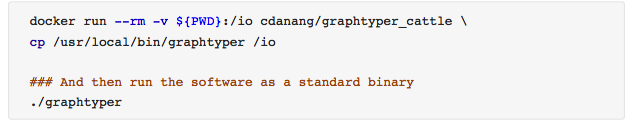
\includegraphics[width=\textwidth]{paper1/supplement/sp12.png}
\end{figure}

If you prefer to modify and build a modified version of Graphtyper for the bovine chromosome
complement directly from the source, please follow the instructions below:

\begin{enumerate}
    \item Clone the \emph{Graphtyper Github}
    \begin{figure}[!htb]
        \centering
        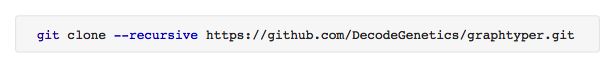
\includegraphics[width=\textwidth]{paper1/supplement/sp13.png}
    \end{figure}

    \item Create a new \emph{branch} at this specific commit tag. We built graphtyper at this specific
    commit hash (04ab5ee460fa36129fb0d8ea5d4b72adc3836f52), to compile at the same
    software version that we use in the paper, please use this commit tag. We named the
    branch as \emph{cattle modification}

    \begin{figure}[!htb]
        \centering
        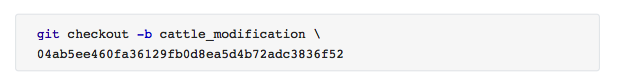
\includegraphics[width=\textwidth]{paper1/supplement/sp14.png}
    \end{figure}

    \item Change directory into \emph{graphtyper} and modify the chromosomal specifications in the files
    include $graphtyper/graph/absolute_position.hpp$ and $src/typer/vcf.cpp$ using UMD 3.1 cattle
    chromosomal names and lengths. The first modification enables all cattle chromosomes
    (esp. for chromosome number $>$ 23) as the current software release set the maximum
    allowed length for each chromosomes according to the human GRChb37 and GRCh38. The
    second modifications are required that the respective chromosomal information is written
    to the \emph{vcf header}.

    \item Make sure that these dependencies are installed:
    \begin{itemize}
        \item C++ compiler with C++11 supported (we tested gcc 4.8.5 or gcc 6.3.0 
        \item Boost$\geq$1.57.0
        \item zlib$\geq$1.2.8
        \item libbz2
        \item liblzma
        \item Autotools, Automake, libtool, Make, and CMake>=2.8.8
    \end{itemize}
    
    \item Follow installation procedures as below. This will put the software in \emph{releasebuild/bin/graphtyper}
    
    \begin{figure}[!htb]
        \centering
        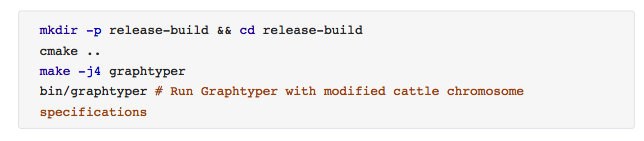
\includegraphics[width=\textwidth]{paper1/supplement/sp15.png}
    \end{figure}

\end{enumerate}

\newpage

\subsection{}
\label{supp_mat:22}
\textbf{\large{Properties of the different metrics used for the evaluation of sequence variant genotyping accuracy.}}


The metrics were calculated using the sum of the red cells as numerator and the cells within the green frame as denominator.
\bigskip
\bigskip
\bigskip

\begin{figure}[!htb]
    \centering
    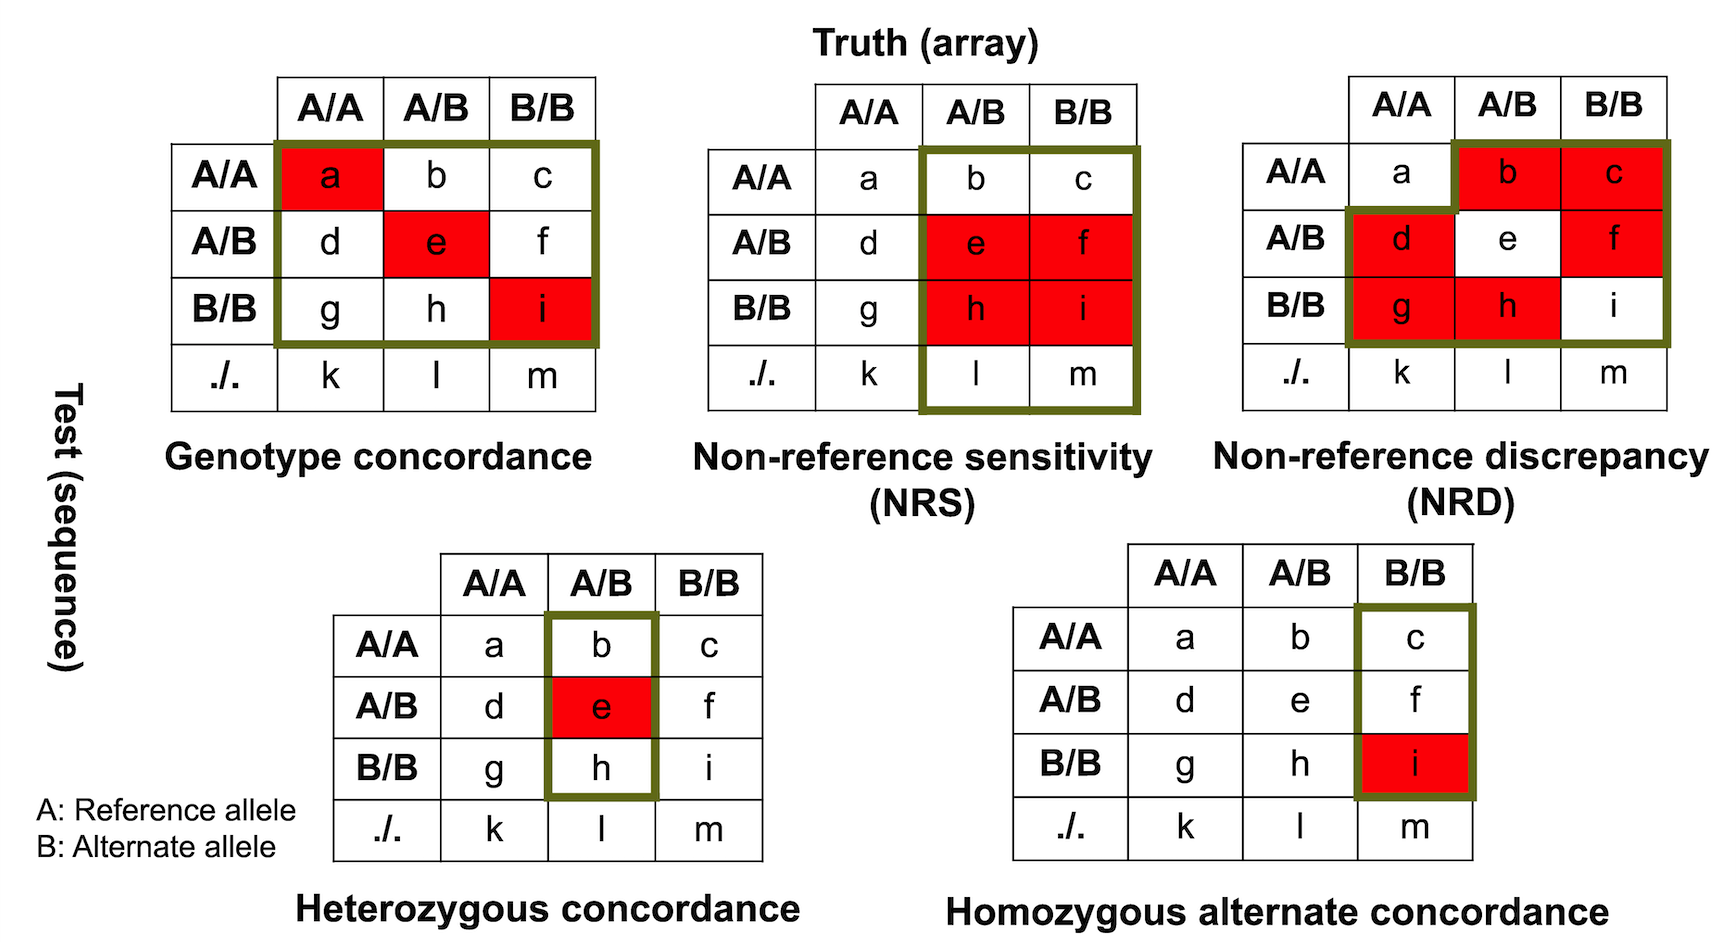
\includegraphics[width=\textwidth]{paper1/supplement/sp2.png}
\end{figure}

\newpage

\begin{landscape}


\subsection{}
\label{supp_mat:23}
\textbf{\large{Concordance statistics}}


The concordance of heterozygous and alternate homozygous genotypes in 49 Original Braunvieh cattle (\textbf{a}) and the concordance at the different sequencing depth for the (\textbf{b}) raw and (\textbf{c}) imputed datasets.

\bigskip
\bigskip
\bigskip

    
    \begin{figure}[!htb]
        \centering
        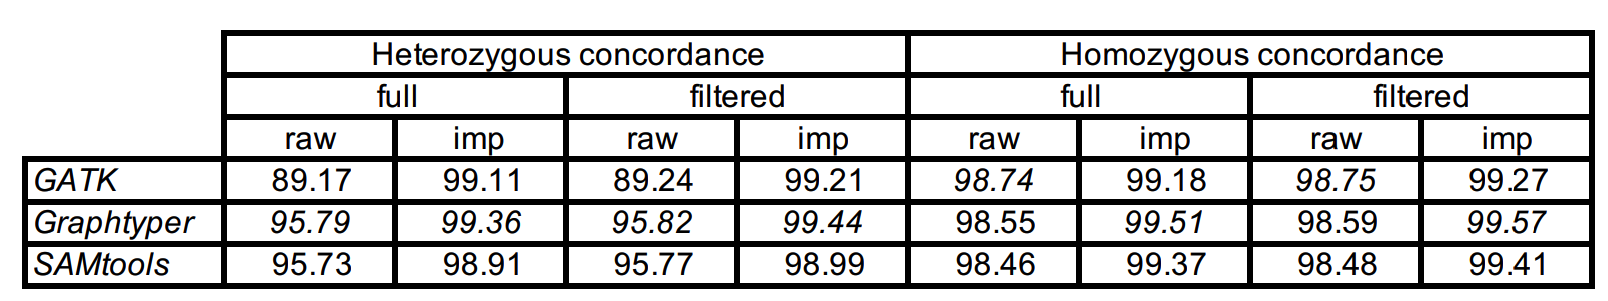
\includegraphics[width=1.4\textwidth]{paper1/supplement/sp31.png}
    \end{figure} 

    \begin{figure}[!htb]
        \centering
        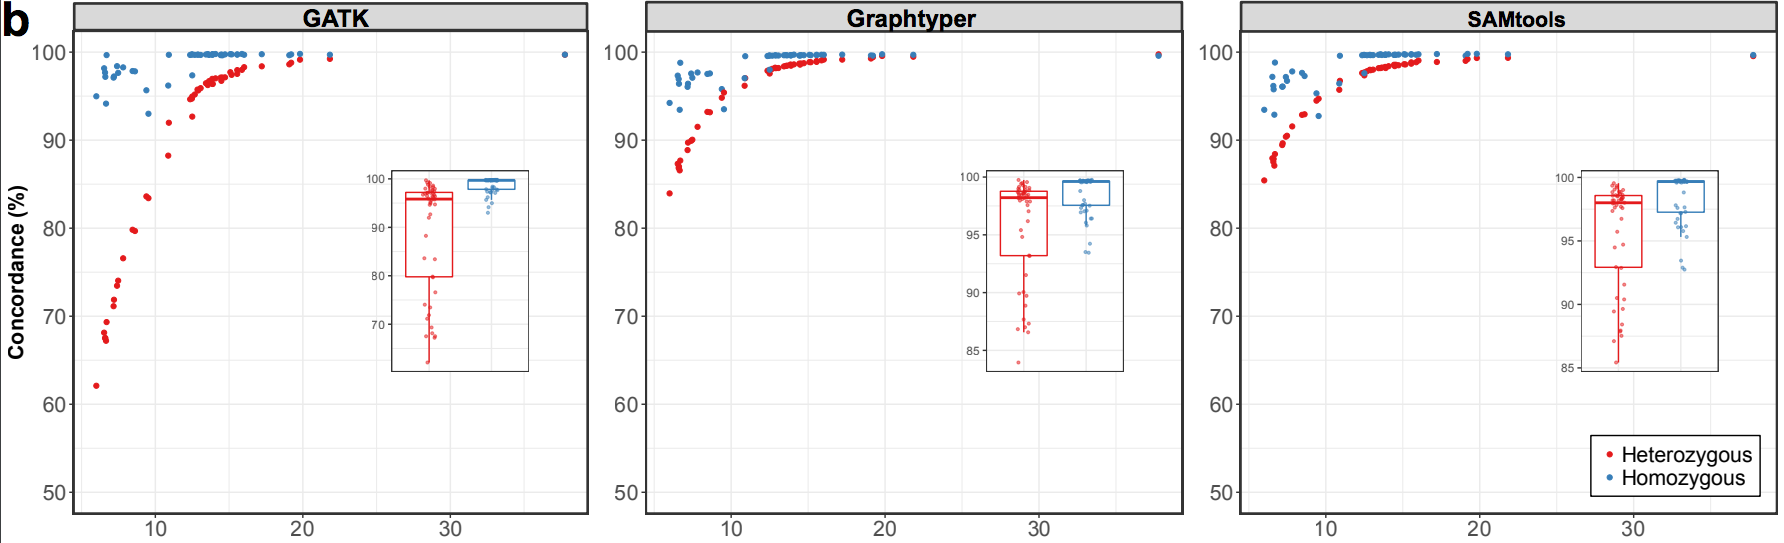
\includegraphics[width=1.5\textwidth]{paper1/supplement/sp32.png}
        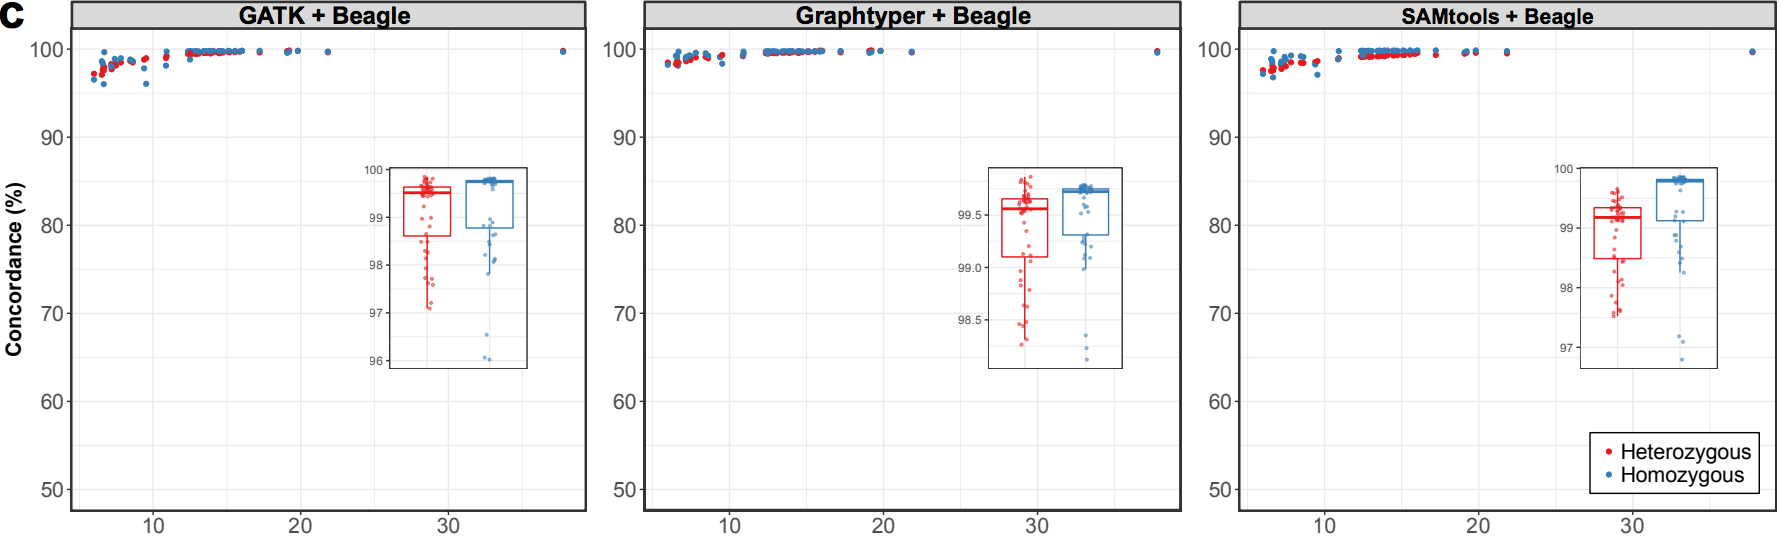
\includegraphics[width=1.5\textwidth]{paper1/supplement/sp33.png}
    \end{figure}

\newpage


\subsection{}
\label{supp_mat:24}
\textbf{\large{Sequence variant genotyping quality for 18 and 31 animals that were sequenced at a lower and higher than 12-fold sequencing coverage, respectively.}}

Asterisks denote significant differences with the best value (italic) for a respective parameter.

\bigskip
\bigskip
\bigskip


    
    \centering
    \emph{Coverage less than 12}
    \begin{footnotesize}
    \arrayrulecolor{black}
    \begin{tabular}{|l|c|c|c|c|c|c|c|c|c|c|c|c|} 
    \cline{2-13}
    \multicolumn{1}{c|}{\multirow{3}{*}{}} & \multicolumn{4}{c|}{Genotype concordance}                 & \multicolumn{4}{c|}{Non-reference sensitivity}            & \multicolumn{4}{c|}{Non-reference discrepancy}             \\ 
    \cline{2-13}
    \multicolumn{1}{c|}{}                  & \multicolumn{2}{c|}{full} & \multicolumn{2}{c|}{filtered} & \multicolumn{2}{c|}{full} & \multicolumn{2}{c|}{filtered} & \multicolumn{2}{c|}{full} & \multicolumn{2}{c|}{filtered}  \\ 
    \cline{2-13}
    \multicolumn{1}{c|}{}                  & raw      & imp~           & raw      & imp                & raw      & imp            & raw      & imp                & raw      & imp            & raw      & imp                 \\ 
    \arrayrulecolor{black}\cline{1-1}\arrayrulecolor{black}\cline{2-13}
    GATK                                   & 90.99*** & 98.7***        & 91.02*** & 98.82***           & 85.63*** & 98.91          & 85.51*** & 98.73              & 14.64*** & 2.09***        & 14.59*** & 1.91***             \\ 
    \hline
    Graphtyper                             & 94.89    & 99.07          & 94.91    & 99.17              & 96.44    & 99             & 96.13    & 98.71              & 8.04     & 1.49           & 8        & 1.31                \\ 
    \hline
    SAMtools                               & 94.87    & 98.61***       & 94.89    & 98.67***           & 96.24*** & 98.94          & 95.75*** & 98.45***           & 8.11     & 2.24***        & 8.09     & 2.11***             \\
    \hline
    \end{tabular}
    \end{footnotesize}


\bigskip
\bigskip

    \centering
    \emph{Coverage more than 12}
    \begin{footnotesize}
    \arrayrulecolor{black}
    \begin{tabular}{|l|c|c|c|c|c|c|c|c|c|c|c|c|} 
    \cline{2-13}
    \multicolumn{1}{c|}{\multirow{3}{*}{}} & \multicolumn{4}{c|}{Genotype concordance}                 & \multicolumn{4}{c|}{Non-reference sensitivity}            & \multicolumn{4}{c|}{Non-reference discrepancy}             \\ 
    \cline{2-13}
    \multicolumn{1}{c|}{}                  & \multicolumn{2}{c|}{full} & \multicolumn{2}{c|}{filtered} & \multicolumn{2}{c|}{full} & \multicolumn{2}{c|}{filtered} & \multicolumn{2}{c|}{full} & \multicolumn{2}{c|}{filtered}  \\ 
    \cline{2-13}
    \multicolumn{1}{c|}{}                  & raw      & imp~           & raw      & imp                & raw     & imp             & raw      & imp                & raw     & imp             & raw     & imp                  \\ 
    \arrayrulecolor{black}\cline{1-1}\arrayrulecolor{black}\cline{2-13}
    GATK                                   & 98.73*** & 99.66          & 98.76*** & 99.71              & 98.3*** & 99.61           & 98.14*** & 99.39              & 1.8***  & 0.48*           & 1.76*** & 0.42                 \\ 
    \hline
    Graphtyper                             & 99.26    & 99.67          & 99.3     & 99.72              & 99.25   & 99.54***        & 98.88    & 99.16***           & 1.04    & 0.45            & 0.99    & 0.4                  \\ 
    \hline
    SAMtools                               & 99.21*** & 99.59***       & 99.24*** & 99.62***           & 99.21** & 99.58***        & 98.51*** & 98.79***           & 1.12*** & 0.58***         & 1.08*** & 0.54***              \\
    \hline
    \end{tabular}
    \end{footnotesize}


\end{landscape}

\newpage

\subsection{}
\label{supp_mat:25}
\textbf{\large{Twelve 1-Mb regions for which \emph{Graphtyper} initially failed to genotype sequence variants}}

The algorithm either ran out of memory or exceeded the allocated runtime (12 h). Graphtyper eventually produced genotypes for the sequence variants when these regions were re-run in 10-kb segments.

\bigskip
\bigskip
\bigskip

\begin{center}
    \begin{tabular}{|c|c|c|} 
        \hline
        No & Chromosome & Region (Mb)  \\ 
        \hline
        1  & 1          & 0-1          \\ 
        \hline
        2  & 1          & 145-146      \\ 
        \hline
        3  & 3          & 69-70        \\ 
        \hline
        4  & 7          & 58-57        \\ 
        \hline
        5  & 8          & 110-111      \\ 
        \hline
        6  & 12         & 76-77        \\ 
        \hline
        7  & 23         & 26-27        \\ 
        \hline
        8  & 23         & 29-30        \\ 
        \hline
        9  & 26         & 50-51        \\ 
        \hline
        10 & 27         & 37-38        \\ 
        \hline
        11 & 28         & 39-40        \\ 
        \hline
        12 & 29         & 30-31        \\
        \hline
        \end{tabular}
\end{center}

\newpage
\subsection{}
\label{supp_mat:26}
\textbf{\large{Variant filtration using \emph{GATK}}}
\bigskip

The best practice guidelines for variant discovery using \emph{GATK} recommend sequence
variants to be filtered using Variant Quality Score Recalibration (VQSR) because it
implements advanced machine learning-based methods to differentiate between true and
false-positive variants. However, VQSR relies on sets of high confidence truth/training
variants, which are currently not (publicly) available in cattle. Thus, we ran \emph{GATK} with best
practice recommendations for variant filtering when applying VQSR is not possible, i.e., we
used a generic baseline hard-filtering threshold for each variant annotation (see
\url{https://gatkforums.broadinstitute.org/GATK/discussion/2806/howto-apply-hard-filters-to-acall-set}). This threshold-based filtering is commonly applied the cattle genomics community
\citep{koufariotis2018sequencing,chen2018whole}
\bigskip



To facilitate running the VQSR module in sheep and goat, i.e., species where sets of
truth/training variants are not (publicly) available, \citep{alberto2018convergent} used an
intersection of high confidence variants that had been discovered from multiple variant
callers as truth/training sets, i.e., they derived truth/training sets directly from the analyzed
data. We implemented their approach to apply \emph{GATK} VQSR to our variant dataset. Training
and truth sets were constructed using the overlap of the filtered variants from the GATK,
\emph{Graphtyper} and \emph{SAMtools} pipelines (truth=false, training=true, known=false, prior= 10) and
markers from the BovineHD BeadChip (truth=true, training=true, known=false, prior= 15),
respectively. Moreover, we used variants listed in dbSNP (version 150) as known variants
(truth=false, training=false, known=true, prior=3.0). Following \emph{GATK} VQSR, we retained
variants in the 99.9\% tranche sensitivity threshold (best practice).

\bigskip

Variant filtration using \emph{GATK} VQSR removed more variants from the raw data than \emph{GATK}
hard filtering (Table 1). However, VQSR retained more HD SNPs than \emph{GATK} hard filtering,
possibly reflecting bias that results from the use of HD SNPs as training/truth sets. The
values of the concordance statistics (genotype concordance, non-reference sensitivity, nonreference discrepancy) were almost identical between \emph{GATK} VQSR and \emph{GATK} hard
filtration (Table 2) indicating that the choice of either filtration option does not notably affect
the concordance between sequence-derived and BovineHD SNP array-derived genotypes.
These findings are in line with \citep{vander2018best} who showed that the concordance
between microarray-called and sequence-derived genotypes is almost identical using either
\emph{GATK} VQSR or the \emph{GATK} 1000 bull genomes project hard filters, even though they used
stringently filtered truth/training sets based on a more comprehensive catalogue of variants
than in our study. Interestingly, in agreement with \citep{vander2018best}, the proportion
of opposing homozygous genotypes in sire/son-pairs (which does not suffer from
ascertainment bias because it is calculated using sequence-derived SNPs) is less using
\emph{GATK} hard filter than \emph{GATK} VQSR.

\bigskip

The performance of \emph{GATK} VQSR may be assessed using the novel variant sensitivity
tranche plot (Figure 2). In the lowest 90\% tranches (highest specificity) the filtering model
still retained many false positive variants (orange box and low Ti/Tv ratio). However, when
the 99.9\% tranche sensitivity is used as filtration criterion as recommended by the \emph{GATK}
best practice guidelines, a high proportion of true positive variants is removed from the
data. 

Overall, our findings suggest that

\begin{enumerate}[(i)]
    \item \emph{GATK} VQSR removes more variants from the data than \emph{GATK} hard filtering,
    \item \emph{GATK} VQSR does not notably improve the concordance between sequencederived and microarray-called genotypes compared to \emph{GATK} hard filtering,
    \item the proportion of opposing homozygous genotypes in sire/son-pairs is higher using \emph{GATK} VQSR than \emph{GATK} hard filtering, and
    \item improving VQSR may be possible by providing more sophisticated truth/training variant datasets produced by orthogonal sequencing technology other than the ones used for training, e.g. \citep{li2018synthetic}
\end{enumerate}

\textbf{Table 1} Comparison of variants statistics between unfiltered and filtered datasets using
either hard-filtering or VQSR.


\bigskip

\begin{center}
\begin{tabular}{|l|l|l|l|} 
    \cline{2-4}
    \multicolumn{1}{l|}{~} & \textit{GATK} full & \textit{GATK }hard-filter & \textit{GATK} VQSR  \\ 
    \hline
    Total SNPs             & 18,594,182         & 17,248,593                & 16,537,577          \\ 
    \hline
    Biallelic              & 18,347,962         & 17,111,806                & 16,430,734          \\ 
    \hline
    Multi-allelic          & 246,220            & 136,787                   & 106,843             \\ 
    \hline
    Ti/Tv ratio            & 2.09               & 2.17                      & 2.16                \\ 
    \hline
    BovineHD               & 99.46              & 99.21                     & 99.38               \\ 
    \hline
    BovineSNP50            & 99.14              & 98.91                     & 98.98               \\
    \hline
    \end{tabular}
\end{center}

\bigskip

\textbf{Table 2} The concordance statistics between hard-filtered and VQSR 

\bigskip

\begin{tabular}{|c|c|c|c|c|} 
    \cline{2-5}
    \multicolumn{1}{c|}{~}    & \begin{tabular}[c]{@{}c@{}}Genotype \\concordance\end{tabular} & \begin{tabular}[c]{@{}c@{}}Non-reference \\sensitivity\end{tabular} & \begin{tabular}[c]{@{}c@{}}Non-reference \\discrepancy\end{tabular} & \begin{tabular}[c]{@{}c@{}}Opposing\\Homozygous\end{tabular}  \\ 
    \hline
    \textit{GATK} hard-filter & 96.02                                                          & 93.67                                                               & 6.3                                                                 & 0.72                                                          \\ 
    \hline
    \textit{GATK} VQSR        & 96.01                                                          & 93.77                                                               & 6.32                                                                & 0.75                                                          \\
    \hline
\end{tabular}

\bigskip
\bigskip


\textbf{Figure 1} Tranche sensitivity plot of novel variants as reported by the VQSR model fitting

\begin{figure}[!htb]
    \centering
    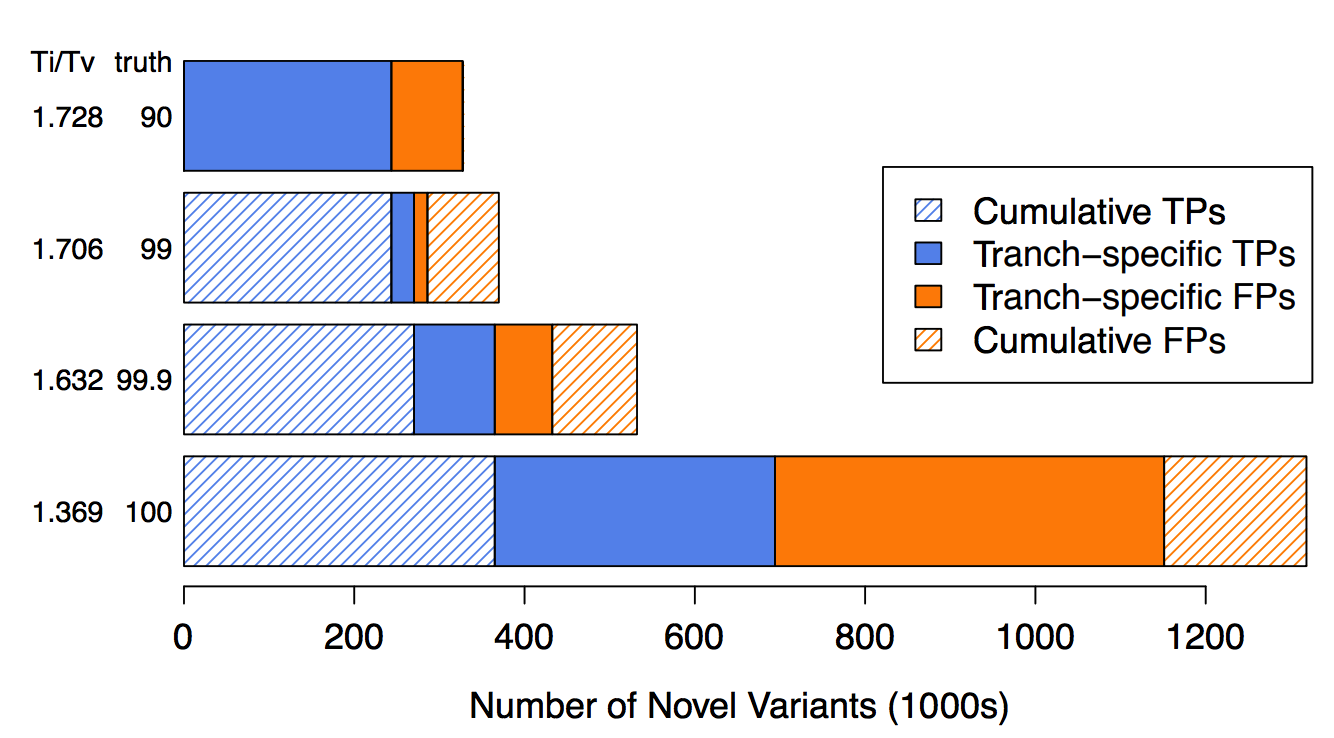
\includegraphics[width=\textwidth]{paper1/supplement/sp6.png}
\end{figure}

\newpage

\begin{landscape}
\subsection{}
\label{supp_mat:27}
\textbf{\large{Accuracy and sensitivity of sequence variant genotyping on bovine chromosome 25 from a variation-aware genome graph that incorporated 2,143,417 dbSNP variants as prior known variants.}}
\bigskip


    \begin{figure}[!htb]
        \centering
        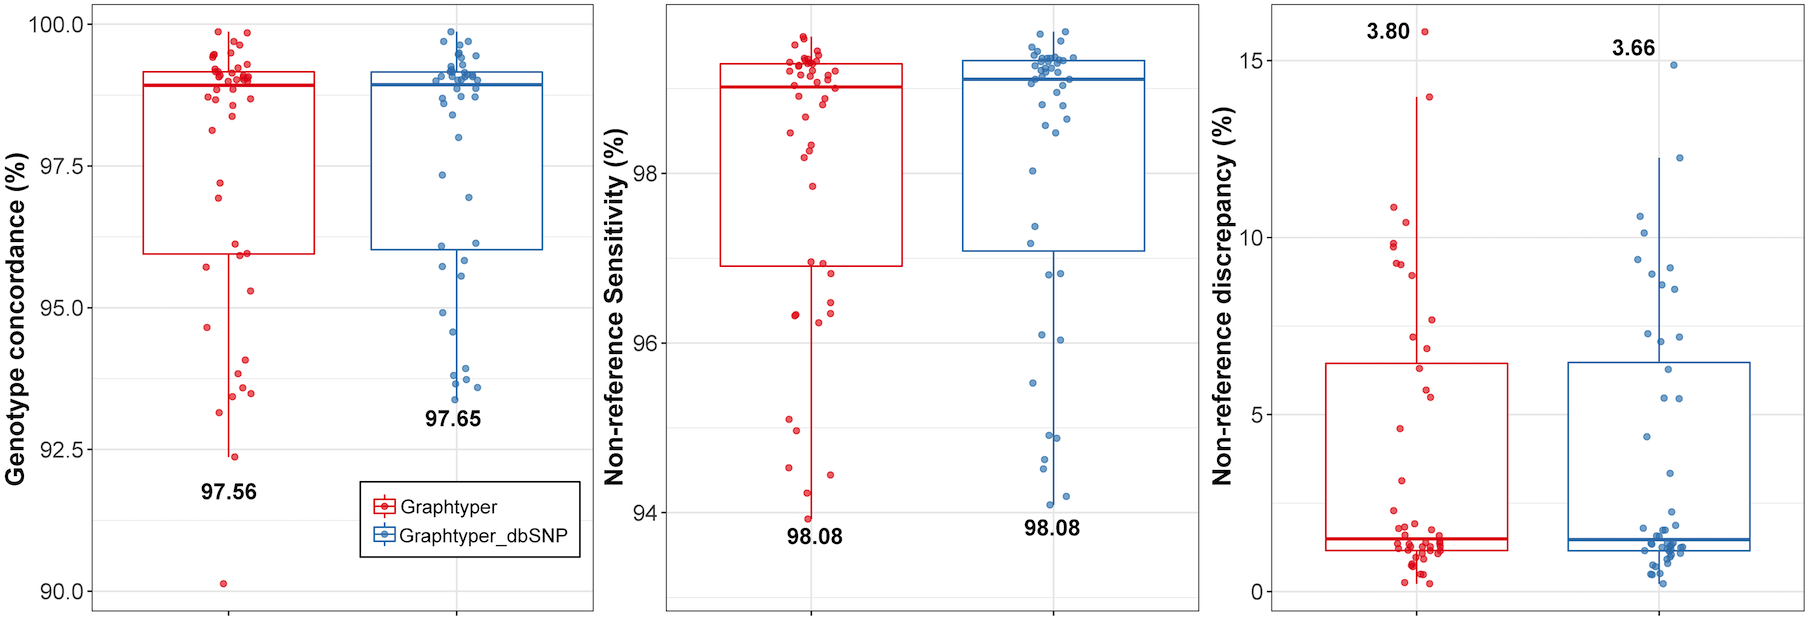
\includegraphics[width=1.5\textwidth]{paper1/supplement/sp7.png}
    \end{figure}
\end{landscape}


\renewcommand{\bibname}{Supplementary References}
\bibliographystyle{abbrvnat}
\bibliography{references/chapter2_ref}

\end{flushleft}

\ifdefined\BuildingFromMainFile
\else
   \end{document}
\fi
